\documentclass[11pt,a4paper]{article}

\usepackage[margin=2.2cm]{geometry}
\usepackage{amsmath,amssymb,amsthm}
\usepackage{booktabs}
\usepackage{array}
\usepackage{tabularx}
\usepackage[shortlabels]{enumitem}
\usepackage{xcolor}
\usepackage{tikz}
\usepackage{fancyhdr}
\usepackage{setspace}
\usepackage{microtype}
\usepackage{titlesec}
\usepackage{hyperref}
\usepackage[skins,breakable]{tcolorbox}

\usetikzlibrary{positioning,arrows.meta,calc,fit,shapes.geometric,matrix,decorations.pathreplacing}

\definecolor{ink}{HTML}{222222}
\definecolor{rulegray}{HTML}{444444}
\definecolor{boxline}{HTML}{666666}
\definecolor{boxfill}{HTML}{F4F4F4}
\definecolor{boxtitle}{HTML}{E8E8E8}
\definecolor{g1}{HTML}{D0D0D0}
\definecolor{g2}{HTML}{9A9A9A}
\definecolor{g3}{HTML}{5A5A5A}

\hypersetup{
  colorlinks=true,
  linkcolor=black,
  urlcolor=black,
  pdftitle={MTL 458 Lecture 14: Advanced Paging},
  pdfauthor={Minati De, IIT Delhi}
}

\setstretch{1.12}
\raggedbottom
\setlist[itemize]{leftmargin=1.3em,itemsep=0.28em,topsep=0.35em}
\setlist[enumerate]{leftmargin=1.5em,itemsep=0.35em,topsep=0.4em}

\titleformat{\section}
  {\Large\bfseries\color{ink}}{\thesection.}{0.6em}{}
  [{\color{rulegray}\titlerule[0.5pt]}]
\titleformat{\subsection}
  {\large\bfseries\color{ink}}{\thesubsection}{0.55em}{}
\titleformat{\subsubsection}
  {\normalsize\bfseries\color{ink}}{\thesubsubsection}{0.5em}{}

\titlespacing*{\section}{0pt}{1.35em}{0.7em}
\titlespacing*{\subsection}{0pt}{1.05em}{0.45em}

\pagestyle{fancy}
\fancyhf{}
\renewcommand{\headrulewidth}{0.4pt}
\renewcommand{\footrulewidth}{0.3pt}
\fancyhead[L]{\small\color{ink}MTL 458 \textbullet\ Operating Systems}
\fancyhead[R]{\small\color{ink}Lecture 14: Advanced Paging}
\fancyfoot[C]{\small\thepage}
\setlength{\headheight}{14pt}

% ---------------------------------------------------------------------------
% Boxes
% ---------------------------------------------------------------------------
\tcbset{
  commonbox/.style={
    colback=boxfill, colframe=boxline, boxrule=0.5pt,
    left=6pt, right=6pt, top=5pt, bottom=5pt,
    fonttitle=\bfseries, coltitle=black, colbacktitle=boxtitle,
    enhanced, sharp corners=south
  }
}
\newtcolorbox{keybox}[1][]{commonbox, title={#1}}
\newtcolorbox{quizbox}[1][]{commonbox, title={#1}}
\newtcolorbox{solbox}[1][]{commonbox, title={#1}}
\newtcolorbox{warnbox}[1][]{commonbox, title={#1}}
\newtcolorbox{defbox}[1][]{commonbox, title={#1}}

\newcommand{\va}{\textit{VA}}
\newcommand{\pa}{\textit{PA}}
\newcommand{\vpn}{\textit{VPN}}
\newcommand{\pfn}{\textit{PFN}}
\newcommand{\ppn}{\textit{PPN}}
\newcommand{\pte}{\textit{PTE}}
\newcommand{\pde}{\textit{PDE}}

% Address-split bar
\newcommand{\addrbar}[3]{%
\begin{center}
\begin{tikzpicture}[x=1cm,y=0.55cm]
  \fill[black!8] (0,0) rectangle (3.4,1);
  \fill[black!16] (3.4,0) rectangle (6.8,1);
  \fill[black!24] (6.8,0) rectangle (12.2,1);
  \draw[black!45] (0,0) rectangle (12.2,1);
  \draw[black!45] (3.4,0) -- (3.4,1);
  \draw[black!45] (6.8,0) -- (6.8,1);
  \node[font=\small\bfseries] at (1.7,0.5) {#1};
  \node[font=\small\bfseries] at (5.1,0.5) {#2};
  \node[font=\small\bfseries] at (9.5,0.5) {#3};
\end{tikzpicture}
\end{center}}

\begin{document}

% ===========================================================================
% Title
% ===========================================================================
\begin{center}
{\color{rulegray}\rule{\textwidth}{1.1pt}}\\[0.45em]
{\LARGE\bfseries Operating Systems}\\[0.25em]
{\Large\bfseries MTL 458 \textperiodcentered\ Lecture 14}\\[0.35em]
{\LARGE\bfseries Advanced Paging}\\[0.35em]
{\large Minati De}\\[0.15em]
{\normalsize Department of Mathematics, Indian Institute of Technology Delhi}\\[0.35em]
{\color{rulegray}\rule{\textwidth}{1.1pt}}
\end{center}

\vspace{0.4em}
\begin{keybox}[What this lecture solves]
Linear page tables fix external fragmentation, but they are
\textbf{too big} and must sit in a \textbf{contiguous} chunk of memory.
Today we shrink and restructure the page table:
\begin{itemize}
  \item \textbf{Inverted page tables} --- one entry per \emph{physical} frame.
  \item \textbf{Segmented page tables} --- one (smaller) table per segment.
  \item \textbf{Multi-level page tables} --- page the page table itself.
\end{itemize}
The TLB from the previous lecture remains the way we hide the extra
lookups. Here the focus is \emph{space}, not time.
\end{keybox}

\tableofcontents
\vspace{0.6em}
{\color{rulegray}\rule{\textwidth}{0.4pt}}

% ===========================================================================
\section{Disadvantages of paging}
% ===========================================================================

Paging gave us a uniform, relocatable address space with no external
fragmentation. Two costs remain.

\subsection{Time: an extra memory reference}
To turn a virtual address into a physical one the MMU must first read a
page-table entry. That is an extra DRAM access on \emph{every} load and
store.
\begin{itemize}
  \item The page table itself lives in memory.
  \item The MMU stores only the \emph{base} of the page table
        (e.g.\ CR3 / PDBR), not the translations.
  \item The previous lecture's fix: a \textbf{TLB}. On a hit, no page-table
        walk is needed.
\end{itemize}

\subsection{Space: the page table can be huge}
A simple (linear) page table stores one \pte\ for \emph{every} virtual
page, allocated or not.
\begin{itemize}
  \item An entry is required even if that page was never touched.
  \item This is painful once the heap and stack grow dynamically and leave
        a large unused hole in the middle of the address space.
\end{itemize}

\begin{warnbox}[Today's problem]
TLBs hide the \emph{time} cost of a page-table lookup.
They do \textbf{not} shrink the page table.
We still need a better data structure for the translations themselves.
\end{warnbox}

% ===========================================================================
\section{How big are page tables?}
% ===========================================================================

A linear page table is an array indexed by \vpn. The number of
slots is the number of virtual pages, not the number of virtual
\emph{bytes}:
\[
  \#\text{virtual pages}
  \;=\;
  \frac{\text{size of VAS}}{\text{page size}}
  \;=\;
  2^{\,(\text{VA bits}\,-\,\lg(\text{page size}))}.
\]
The low \(\lg(\text{page size})\) bits are the page offset; they never
index the page table. Then
\[
  \text{page-table size}
  \;=\;
  (\text{\pte\ size})
  \times
  (\#\text{virtual pages}).
\]
The whole array must sit in one contiguous physical region, because
hardware finds \pte\ \(\vpn\) by
\(\textit{base} + \vpn \times (\text{\pte\ size})\).

\begin{quizbox}[Quiz --- size of a linear page table]
Compute the size of a single process's linear page table.
\end{quizbox}

\begin{solbox}[Worked answers]
\begin{enumerate}[leftmargin=1.4em]
  \item \textbf{\pte s are 2\,B, and there are 32 possible VPNs.}
  \[
    32 \times 2\,\text{B} = 64\,\text{B}.
  \]
  Tiny --- a 5-bit VPN world.

  \item \textbf{\pte s are 2\,B, VA is 24 bits, pages are 16\,B.}
  \[
    \text{offset bits}=\lg 16=4,
    \quad
    \#\text{VPNs}=2^{24-4}=2^{20},
    \quad
    2 \times 2^{20} = 2^{21}\,\text{B} = 2\,\text{MB}.
  \]

  \item \textbf{\pte s are 4\,B, VA is 32 bits, pages are 4\,KB.}
  \[
    \text{offset bits}=\lg(4\,\text{KB})=12,
    \quad
    \#\text{VPNs}=2^{20},
    \quad
    4 \times 2^{20} = 2^{22}\,\text{B} = 4\,\text{MB}.
  \]
  Four megabytes of contiguous kernel memory \emph{per process}, most of
  it unused.

  \item \textbf{\pte s are 4\,B, VA is 64 bits, pages are 4\,KB.}
  \[
    \#\text{VPNs}=2^{64-12}=2^{52},
    \quad
    4 \times 2^{52} = 2^{54}\,\text{B}
    \;=\; 16\,\text{PB}.
  \]
  Impossible as a linear array. This is why 64-bit machines \emph{must}
  use multi-level (or hashed) page tables.
\end{enumerate}
\end{solbox}

% ===========================================================================
\section{Why linear page tables waste so much space}
% ===========================================================================

A typical process does not use its address space densely. Code and heap
sit at the low end; the stack sits at the high end; almost everything
in between is unused.

\begin{center}
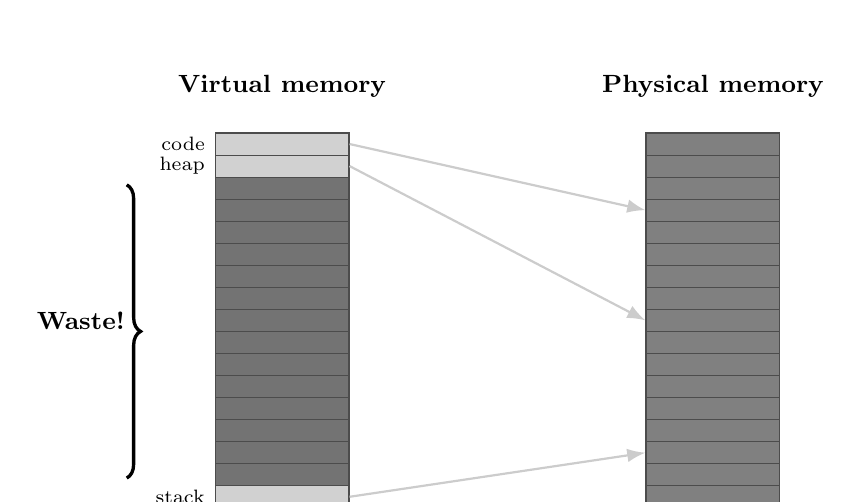
\begin{tikzpicture}[
  x=0.72cm, y=0.28cm,
  slot/.style={draw=black!70, minimum width=1.7cm, minimum height=0.28cm,
               inner sep=0, font=\scriptsize},
  used/.style={slot, fill=black!18},
  unused/.style={slot, fill=black!55},
  phys/.style={slot, fill=black!50},
  arr/.style={-{Latex}, thick, white!80!black}
]
  \node[font=\small\bfseries] at (1.0, 18.6) {Virtual memory};
  \node[font=\small\bfseries] at (8.6, 18.6) {Physical memory};

  % virtual column
  \foreach \y in {0,...,16} {
    \node[unused] (v\y) at (1.0, \y) {};
  }
  \node[used] (v16) at (1.0, 16) {};
  \node[used] (v15) at (1.0, 15) {};
  \node[used] (v0)  at (1.0, 0)  {};

  \node[left, font=\scriptsize] at (v16.west) {code};
  \node[left, font=\scriptsize] at (v15.west) {heap};
  \node[left, font=\scriptsize] at (v0.west)  {stack};

  \draw[black, very thick, decorate, decoration={brace,amplitude=5pt}]
    ($(v14.west)+(-1.55,0.15)$) -- ($(v1.west)+(-1.55,-0.15)$);
  \node[font=\small\bfseries, align=center]
    at (-2.55, 8) {Waste!};

  % physical column
  \foreach \y in {0,...,16} {
    \node[phys] (p\y) at (8.6, \y) {};
  }

  \draw[arr] (v16.east) -- (p13.west);
  \draw[arr] (v15.east) -- (p8.west);
  \draw[arr] (v0.east)  -- (p2.west);
\end{tikzpicture}
\end{center}

Paging still maps used pages to \emph{any} free frames (no external
fragmentation). The unused hole in the middle of the VAS does
\emph{not} waste physical frames --- those pages are simply never
mapped. The waste is in the \textbf{page table}: a linear table
still reserves a slot for every virtual page in the hole, and that
array must be allocated up front.

\subsection{A linear page table is full of invalid entries}

\begin{center}
\renewcommand{\arraystretch}{1.15}
\begin{tabular}{rccc}
  \toprule
  \textbf{VPN} & \textbf{PFN} & \textbf{valid} & \textbf{prot} \\
  \midrule
  0  & 10 & 1 & \texttt{r-x} \\
  1  & -- & 0 & -- \\
  2  & 23 & 1 & \texttt{rw-} \\
  3  & -- & 0 & -- \\
  4  & -- & 0 & -- \\
  5  & -- & 0 & -- \\
     & $\vdots$ & $\vdots$ & \textit{many more invalid} \\
  $N{-}2$ & 28 & 1 & \texttt{rw-} \\
  $N{-}1$ & 4  & 1 & \texttt{rw-} \\
  \bottomrule
\end{tabular}
\end{center}

Valid translations cluster at the two ends (code/heap and stack).
The enormous middle is a run of \(\textit{valid}=0\) entries that we
would like to \textbf{not store at all}.

\begin{keybox}[Observation]
Valid \pte s are \emph{contiguous in clumps}, not sprinkled uniformly.
Any design that can skip a whole unused region of the VPN space will
win.
\end{keybox}

% ===========================================================================
\section{We do not have to use a flat array}
% ===========================================================================

A page table is just a data structure that answers
\[
  (\vpn,\,\textit{ASID}) \;\longmapsto\; (\ppn,\,\textit{prot}).
\]
If the TLB is \textbf{software-managed}, the OS may use \emph{any}
structure it likes.

\begin{itemize}
  \item Hardware looks up the \vpn\ in the TLB on every memory access.
  \item On a miss the CPU traps into the kernel.
  \item The OS finds the translation, fills the TLB, and retries the
        instruction.
\end{itemize}

If instead the \textbf{hardware} walks the page table (x86, ARM, \ldots),
the table must follow a layout the MMU understands --- typically a
radix tree of page-table pages.

\begin{center}
\renewcommand{\arraystretch}{1.12}
\begin{tabular}{@{}lll@{}}
  \toprule
  \textbf{Approach} & \textbf{Core idea} & \textbf{TLB miss handler} \\
  \midrule
  Inverted page table     & one entry per physical frame & software \\
  Segmented page tables   & one table per segment        & either \\
  Multi-level page tables & page the page tables         & hardware (x86) \\
  \bottomrule
\end{tabular}
\end{center}

% ===========================================================================
\section{Approach 1: inverted page tables}
% ===========================================================================

\begin{defbox}[Inverted page table]
Store one entry per \emph{occupied physical frame}, not per virtual
page. The table size tracks \textbf{physical memory}, which is much
smaller than a 64-bit virtual address space.
\end{defbox}

``Inverted'' means the index is flipped. A linear table is
\(\vpn \to \ppn\). An inverted table is stored as
\(\ppn \to (\vpn, \textit{ASID})\): one row per frame, saying which
virtual page (of which process) lives there.

The \textit{ASID} is required because two processes can use the same
\vpn. Without it, a lookup could return another process's frame.

\paragraph{Na\"ive lookup.}
The CPU gives us a \vpn, but the table is indexed by \ppn. So we
must \emph{search}: scan every row for a matching
\((\vpn,\textit{ASID})\). Correct, but \(O(\#\text{frames})\) --- far
too slow for a TLB miss path.

\paragraph{Hashed inverted table.}
Hash \((\vpn,\textit{ASID})\) into a bucket, then search only that
chain. Used on IBM PowerPC-style machines. The table is still
\(O(\text{physical memory})\), but a miss is now roughly \(O(1)\).

\begin{keybox}[Hardware implication]
Managing an inverted / hashed table is awkward for a hardware walker.
It is a natural fit for a \textbf{software-controlled TLB}: the miss
trap lets the OS run an arbitrary lookup, then insert the result.
Hardware-controlled TLBs want a simple, well-defined walk --- which
leads to multi-level page tables.
\end{keybox}

% ===========================================================================
\section{Approach 2: combine paging and segmentation}
% ===========================================================================

Valid pages come in a few clumps (code, heap, stack). So: keep
\textbf{segmentation} for those clumps, and \textbf{page} each clump.

\begin{itemize}
  \item Split the address space into variable-length \emph{segments}
        (code, heap, stack, \ldots).
  \item Split each segment into fixed-size \emph{pages}.
  \item Each segment has its \emph{own} page table.
  \item Hardware tracks, per segment, the \textbf{base} (physical address
        of that segment's page table) and a \textbf{bounds}
        (number of valid \pte s / size of that table).
\end{itemize}

A logical address then has three fields:

\addrbar{seg \# (4 bits)}{page number (8 bits)}{page offset (12 bits)}

This is not the old ``one base+bounds for the whole segment of
bytes.'' \textit{Base} now points at that segment's \emph{page
table}, and \textit{bounds} is how many \pte s that table has
(i.e.\ how many pages the segment currently uses). The unused hole
between heap and stack is simply a segment we never create a table
for.

Translation:
\begin{enumerate}
  \item Use the segment number to select \((\textit{base},\,\textit{bounds})\).
  \item If \(\textit{page number} \ge \textit{bounds}\), segmentation fault
        --- that page is past the end of this segment's table.
  \item \(\pte = \textit{Mem}[\textit{base} + \textit{page number}]\).
  \item If the \pte\ is valid, \(\pa = (\pfn \ll 12) \mid \textit{offset}\).
\end{enumerate}

\subsection{Advantages}

\begin{center}
\renewcommand{\arraystretch}{1.15}
\begin{tabularx}{\textwidth}{@{}lX@{}}
  \toprule
  \textbf{From segments} & Supports sparse address spaces. Unused segments
                           need no page table at all. Each table is only
                           as long as that segment. \\
  \textbf{From pages}    & No external fragmentation. A segment can grow
                           by adding pages, with no reshuffling of other
                           segments. A process can run even if some of
                           its pages have been swapped to disk
                           (next lecture). \\
  \textbf{Together}      & Sparse VAS \emph{and} compact, per-segment
                           tables, with page-granularity placement. \\
  \bottomrule
\end{tabularx}
\end{center}

\subsection{Disadvantages}

Each per-segment page table must still be allocated
\textbf{contiguously}, and it can still be large.

\begin{quizbox}[Size of one segmented page table]
Assume 2 bits of segment number, 18 bits of page number, 12 bits of
offset, and 4-byte \pte s. How big is \emph{one} segment's page table
in the worst case?
\end{quizbox}

\begin{solbox}[Answer]
\[
  2^{18}\ \text{entries}
  \times
  4\,\text{B}
  \;=\;
  2^{20}\,\text{B}
  \;=\;
  1\,\text{MB}.
\]
Up to 1\,MB of \emph{contiguous} memory per segment --- and worse as
the VPN field grows. Segmented paging helps, but it does not solve the
contiguous-allocation problem for large address spaces.
\end{solbox}

% ===========================================================================
\section{Approach 3: multi-level page tables}
% ===========================================================================

\begin{defbox}[Idea --- page the page table]
Treat the linear page table as just another byte array and
\textbf{page it}, the same way we page user memory. Cut the big
array into page-sized chunks. The outer table (the \emph{page
directory}) has one entry per chunk: either ``this chunk exists, here
is its frame'' or ``this whole VPN range is unused --- do not
allocate the chunk.''
\end{defbox}

Consequences:
\begin{itemize}
  \item The page table need not be contiguous in physical memory.
  \item Only regions of the VAS that are actually used consume inner
        page-table pages.
  \item Hardware can walk a fixed radix tree. This is the x86 page-table
        format (2 levels on IA-32, 4--5 levels on x86-64).
\end{itemize}

\subsection{Two-level split of a 30-bit address}

\addrbar{outer page (8 bits)}{inner page (10 bits)}{page offset (12 bits)}

\begin{center}
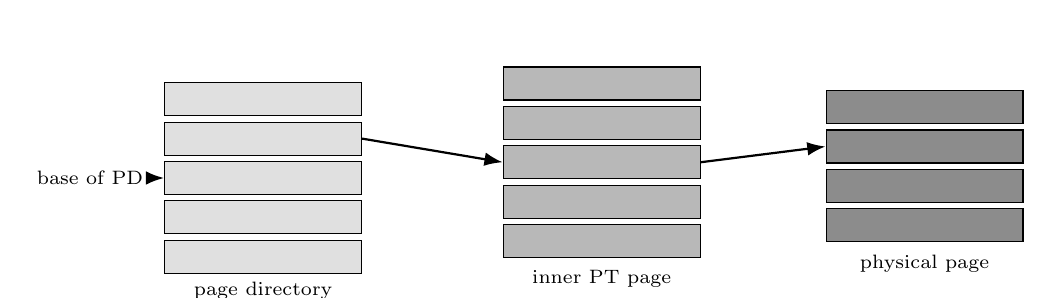
\begin{tikzpicture}[
  every node/.style={font=\small},
  box/.style={draw, minimum width=2.5cm, minimum height=0.42cm, inner sep=1pt},
  dbox/.style={box, fill=black!12},
  ibox/.style={box, fill=black!28},
  mbox/.style={box, fill=black!45},
  arr/.style={-{Latex}, thick}
]
  \node[dbox] (d0) at (0,3.2) {};
  \node[dbox] (d1) at (0,2.7) {};
  \node[dbox] (d2) at (0,2.2) {};
  \node[dbox] (d3) at (0,1.7) {};
  \node[dbox] (d4) at (0,1.2) {};
  \node[anchor=north, font=\scriptsize] at (0,1.0)
        {page directory};
  \node[anchor=east, font=\scriptsize] at (-1.4,2.2)
        {base of PD};

  \node[ibox] (i0) at (4.3,3.4) {};
  \node[ibox] (i1) at (4.3,2.9) {};
  \node[ibox] (i2) at (4.3,2.4) {};
  \node[ibox] (i3) at (4.3,1.9) {};
  \node[ibox] (i4) at (4.3,1.4) {};
  \node[anchor=north, font=\scriptsize] at (4.3,1.15)
        {inner PT page};

  \node[mbox] (m0) at (8.4,3.1) {};
  \node[mbox] (m1) at (8.4,2.6) {};
  \node[mbox] (m2) at (8.4,2.1) {};
  \node[mbox] (m3) at (8.4,1.6) {};
  \node[anchor=north, font=\scriptsize] at (8.4,1.35)
        {physical page};

  \draw[arr] (-1.35,2.2) -- (d2.west);
  \draw[arr] (d1.east) -- (i2.west);
  \draw[arr] (i2.east) -- (m1.west);
\end{tikzpicture}
\end{center}

Think of the \vpn\ as a two-digit page-table address. The high
digit (\textit{outer}) picks a row of the directory; that row names
which inner table to use. The low digit (\textit{inner}) picks a
row of that inner table; that row names the user frame. The offset
is copied through unchanged --- it never goes into either table.

Walk:
\begin{enumerate}
  \item \(\pde = \textit{PD}[\textit{outer}]\). If invalid \(\to\) fault
        (no inner table for this VPN range).
  \item \(\pte = \textit{PT}_{\pde.\ppn}[\textit{inner}]\). If invalid
        \(\to\) fault (this virtual page itself is not mapped).
  \item \(\pa = (\pte.\pfn \ll 12) \mid \textit{offset}\).
\end{enumerate}
A TLB miss now costs \textbf{two} memory references (PD + PT) before
the actual data access --- three in total. The TLB is what makes this
acceptable: after the first miss those two walks are cached, so later
accesses to the same page cost one memory reference again.

\subsection{Linear versus multi-level, side by side}

The figure on the lecture slide (OSTEP Fig.~20.3) makes the saving
concrete. Four \pte s fit in one page-of-page-table.

\begin{center}
\resizebox{\textwidth}{!}{%
\begin{tabular}{@{}ll@{}}
\begin{minipage}[t]{0.46\textwidth}
\centering
\textbf{Linear page table}\\[0.3em]
{\small PDBR \(= 201\)}\\[0.4em]
\renewcommand{\arraystretch}{1.12}
\begin{tabular}{cccc}
  \toprule
  v & prot & PFN & loc \\
  \midrule
  1 & \texttt{r-x} & 12  & \scriptsize PFN 201 \\
  1 & \texttt{r-x} & 13  & \\
  0 & --           & --  & \\
  1 & \texttt{rw-} & 100 & \\
  \midrule
  0 & -- & -- & \scriptsize PFN 202 \\
  0 & -- & -- & \\
  0 & -- & -- & \\
  0 & -- & -- & \\
  \midrule
  0 & --           & -- & \scriptsize PFN 203 \\
  0 & --           & -- & \\
  1 & \texttt{rw-} & 86 & \\
  1 & \texttt{rw-} & 15 & \\
  \bottomrule
\end{tabular}
\end{minipage}
&
\begin{minipage}[t]{0.52\textwidth}
\centering
\textbf{Multi-level page table}\\[0.3em]
{\small PDBR \(= 200\)}\\[0.4em]
\renewcommand{\arraystretch}{1.12}
\begin{tabular}{ccc}
  \toprule
  v & PFN & loc \\
  \midrule
  1 & 201 & \scriptsize PD @ 200 \\
  0 & --  & \\
  0 & --  & \\
  1 & 203 & \\
  \bottomrule
\end{tabular}\\[0.7em]
\renewcommand{\arraystretch}{1.12}
\begin{tabular}{cccc}
  \toprule
  v & prot & PFN & loc \\
  \midrule
  1 & \texttt{r-x} & 12  & \scriptsize PT @ 201 \\
  1 & \texttt{r-x} & 13  & \\
  0 & --           & --  & \\
  1 & \texttt{rw-} & 100 & \\
  \midrule
  \multicolumn{4}{c}{\textit{middle PT page never allocated}} \\
  \midrule
  0 & --           & -- & \scriptsize PT @ 203 \\
  0 & --           & -- & \\
  1 & \texttt{rw-} & 86 & \\
  1 & \texttt{rw-} & 15 & \\
  \bottomrule
\end{tabular}
\end{minipage}
\end{tabular}}
\end{center}

Read the two sides as the same mappings. Linear PDBR \(201\) is one
12-entry array stored in frames \(201,202,203\). Multi-level PDBR
\(200\) is a 4-entry directory: slot 0 points at the first chunk
(still frame \(201\)), slot 3 points at the last chunk (frame
\(203\)), and slot 1 is invalid. The middle chunk (old frame
\(202\)) is a page of invalid \pte s, so it is \textbf{never
allocated}. That is the space saving --- one physical page returned
to the free list --- and it grows with every unused VPN range.

\begin{keybox}[Meaning of the valid bit]
\begin{itemize}
  \item In a \pde: ``does an inner page-table page exist for this VPN
        range?''
  \item In a \pte: ``is this virtual page itself resident / legal?''
\end{itemize}
A fault can happen at \emph{either} level.
\end{keybox}

\subsection{How to slice the address}

The split is not arbitrary. The design goal is:

\begin{quote}
\textit{Each page of page table must fit in one physical page.}
\end{quote}

\begin{quizbox}[Quiz --- address format for two-level paging]
A 30-bit virtual address, 4\,KB pages, 4-byte \pte s.
How many bits for the inner index? How many remain for the outer
(directory) index?
\end{quizbox}

\begin{solbox}[Answer]
\[
  \text{page size}=2^{12}\,\text{B}
  \quad\Rightarrow\quad
  \text{offset}=12\text{ bits}.
\]
We need
\[
  (\text{\pte\ size})\times(\#\pte\text{s per inner page})
  \;=\;
  \text{page size},
\]
so
\[
  4 \times \#\pte\text{s} = 2^{12}
  \quad\Rightarrow\quad
  \#\pte\text{s}=2^{10}
  \quad\Rightarrow\quad
  \textbf{inner index}=10\text{ bits}.
\]
The leftover VPN bits become the directory index:
\[
  30 - 12 - 10 = 8\text{ bits}.
\]
That is exactly the \(8{+}10{+}12\) split drawn above.

Why force the inner table into one page? Then the directory stores
one frame number per inner table, the OS can place each inner table
anywhere, and an unused VPN range costs one invalid directory bit
instead of a whole contiguous array.
\end{solbox}

% ===========================================================================
\section{Quiz: walking a two-level page table}
% ===========================================================================

20-bit virtual addresses, two-level tables:

\addrbar{outer (4 bits)}{inner (4 bits)}{page offset (12 bits)}

A 20-bit address is five hex digits. Split them as
\(0x\,\underbrace{X}_{4\text{ bits}}\,\underbrace{Y}_{4\text{ bits}}\,\underbrace{ZZZ}_{12\text{ bits}}\):
\(\textit{outer}=X\), \(\textit{inner}=Y\), \(\textit{offset}=ZZZ\).
Each table has \(2^{4}=16\) slots (indices \(0x0\)--\(0xF\)).
The physical address is the inner table's \ppn\ with the same
offset glued on: if the \pte\ says frame \(0x23\) and the offset is
\(0xABC\), then \(\pa=0x23ABC\).

\begin{center}
\renewcommand{\arraystretch}{1.08}
\setlength{\tabcolsep}{4pt}
\begin{tabular}{@{}ccc@{}}
\textbf{page directory}
&
\textbf{PT @ PPN \(0x3\)}
&
\textbf{PT @ PPN \(0x92\)} \\[0.3em]
\begin{tabular}{cc}
  \toprule
  PPN & v \\
  \midrule
  \(0x3\)  & 1 \\
  --       & 0 \\
  --       & 0 \\
  --       & 0 \\
  --       & 0 \\
  --       & 0 \\
  --       & 0 \\
  --       & 0 \\
  --       & 0 \\
  --       & 0 \\
  --       & 0 \\
  --       & 0 \\
  --       & 0 \\
  --       & 0 \\
  --       & 0 \\
  \(0x92\) & 1 \\
  \bottomrule
\end{tabular}
&
\begin{tabular}{cc}
  \toprule
  PPN & v \\
  \midrule
  \(0x10\) & 1 \\
  \(0x23\) & 1 \\
  --       & 0 \\
  --       & 0 \\
  \(0x80\) & 1 \\
  \(0x59\) & 1 \\
  --       & 0 \\
  --       & 0 \\
  --       & 0 \\
  --       & 0 \\
  --       & 0 \\
  --       & 0 \\
  --       & 0 \\
  --       & 0 \\
  --       & 0 \\
  --       & 0 \\
  \bottomrule
\end{tabular}
&
\begin{tabular}{cc}
  \toprule
  PPN & v \\
  \midrule
  --       & 0 \\
  --       & 0 \\
  --       & 0 \\
  --       & 0 \\
  --       & 0 \\
  --       & 0 \\
  --       & 0 \\
  --       & 0 \\
  --       & 0 \\
  --       & 0 \\
  --       & 0 \\
  --       & 0 \\
  --       & 0 \\
  --       & 0 \\
  \(0x55\) & 1 \\
  \(0x45\) & 1 \\
  \bottomrule
\end{tabular}
\end{tabular}
\end{center}

\begin{quizbox}[Translate these virtual addresses]
(a) \(0x01ABC\) \qquad (b) \(0x00000\) \qquad (c) \(0xFEED0\)\\[0.2em]
Also useful: \(0x04000\).
\end{quizbox}

\begin{solbox}[Walk]
\paragraph{(a) \(0x01ABC \to 0x23ABC\).}
Outer \(=0x0\), inner \(=0x1\), offset \(=0xABC\).
\[
  \textit{PD}[0]=0x3\ (\text{valid})
  \;\to\;
  \textit{PT}_{0x3}[1]=0x23\ (\text{valid})
  \;\to\;
  \pa=0x23ABC.
\]

\paragraph{(b) \(0x00000 \to 0x10000\).}
Outer \(=0x0\), inner \(=0x0\), offset \(=0x000\).
\[
  \textit{PD}[0]=0x3
  \;\to\;
  \textit{PT}_{0x3}[0]=0x10
  \;\to\;
  \pa=0x10000.
\]

\paragraph{(c) \(0xFEED0 \to 0x55ED0\).}
Outer \(=0xF\), inner \(=0xE\), offset \(=0xED0\).
\[
  \textit{PD}[0xF]=0x92\ (\text{valid})
  \;\to\;
  \textit{PT}_{0x92}[0xE]=0x55\ (\text{valid})
  \;\to\;
  \pa=0x55ED0.
\]

\paragraph{Bonus: \(0x04000 \to 0x80000\).}
Outer \(=0x0\), inner \(=0x4\), offset \(=0x000\).
\[
  \textit{PD}[0]=0x3
  \;\to\;
  \textit{PT}_{0x3}[4]=0x80
  \;\to\;
  \pa=0x80000.
\]
Any other outer index except \(0x0\) and \(0xF\) faults immediately
(directory miss). Inner indices \(0x2,0x3,0x6,\ldots\) of \(\textit{PT}_{0x3}\)
fault even though the directory slot is valid.
\end{solbox}

% ===========================================================================
\section{When two levels are not enough}
% ===========================================================================

The same ``one table = one page'' rule applies to the directory.
If the leftover outer index is wider than
\(\lg(\text{page size}/\text{\pte\ size})\), the directory itself
spills across many pages, and we are back to a contiguous allocation
problem --- just one level up.

\begin{warnbox}[Example --- directory no longer fits]
30-bit \va, 512-byte pages, 4-byte \pte s.
\begin{itemize}
  \item Offset \(=\lg 512=9\) bits, so \(\vpn\) has 21 bits.
  \item Entries per page \(=512/4=128=2^{7}\) \(\Rightarrow\) inner index
        \(=7\) bits.
  \item Outer index \(=21-7=14\) bits \(\Rightarrow\) \(2^{14}\) directory
        entries.
  \item Directory size \(=2^{14}\times 4\,\text{B}=64\,\text{KB}=128\) pages.
\end{itemize}
The ``page directory'' is no longer one page. Solution: \textbf{page the
page directory} --- add another level.
\end{warnbox}

\addrbar{PD idx 0}{PD idx 1  +  PT idx}{offset}

In the limit this is just a radix tree of page-table pages. x86-64 uses
four (now five) such levels.

\subsection{How large a VAS can \texorpdfstring{\(L\)}{L} levels cover?}

Keep the usual 4\,KB page and 4-byte \pte. Then every level has
\[
  \frac{4\,\text{KB}}{4\,\text{B}} = 1024 = 2^{10}
\]
slots, and the offset is 12 bits.

\begin{center}
\renewcommand{\arraystretch}{1.2}
\begin{tabular}{cccc}
  \toprule
  \textbf{Levels} & \textbf{Bit split} & \textbf{VAS size} & \textbf{Approx.} \\
  \midrule
  1 & \(10+12\)           & \(2^{10}\times 4\,\text{KB}=2^{22}\) & 4\,MB \\
  2 & \(10+10+12\)        & \(2^{20}\times 4\,\text{KB}=2^{32}\) & 4\,GB \\
  3 & \(10+10+10+12\)     & \(2^{30}\times 4\,\text{KB}=2^{42}\) & 4\,TB \\
  \bottomrule
\end{tabular}
\end{center}

A full 64-bit space with 4\,KB pages and 4-byte \pte s needs
\(\lceil 52/10\rceil=6\) levels (or 8-byte \pte s and a 4-level canonical
48-bit x86-64 layout). The lecture's point: \emph{keep adding levels
until the top table fits in one page}.

\begin{warnbox}[Cost of depth]
On a TLB miss the walker touches one page-table page per level, then
the data page. A 3-level table turns one miss into \textbf{4} memory
references. That is why a large, high-hit-rate TLB is not optional.
\end{warnbox}

% ===========================================================================
\section{Quiz: the full system with a TLB}
% ===========================================================================

\begin{quizbox}[Setup]
\begin{itemize}
  \item 3-level page table (so a miss costs \textbf{3} PT memory accesses).
  \item 256-byte pages, 16-bit virtual addresses
        \(\Rightarrow\) \(\vpn\) is the high 8 bits, offset the low 8 bits.
  \item Current process \textit{ASID} \(=2111\).
  \item Count \emph{physical memory accesses} per instruction.
        Ignore the fact that a fill changes the TLB for later ops.
\end{itemize}

\begin{center}
\renewcommand{\arraystretch}{1.12}
\begin{tabular}{cccc}
  \toprule
  \textbf{ASID} & \textbf{VPN} & \textbf{PFN} & \textbf{valid} \\
  \midrule
  2111 & \(0\text{xbb}\) & \(0\text{x91}\) & 1 \\
  2111 & \(0\text{xff}\) & \(0\text{x23}\) & 1 \\
  1222 & \(0\text{x05}\) & \(0\text{x91}\) & 1 \\
  2111 & \(0\text{x05}\) & \(0\text{x12}\) & 0 \\
  \bottomrule
\end{tabular}
\end{center}

\begin{enumerate}[(a)]
  \item \(0\text{xAA10}\):\quad \texttt{movl 0x1111, \%edi}
  \item \(0\text{xBB13}\):\quad \texttt{addl \$0x3, \%edi}
  \item \(0\text{x0519}\):\quad \texttt{movl \%edi, 0xFF10}
\end{enumerate}
\end{quizbox}

\begin{solbox}[Access counts]
Every instruction needs its bytes fetched from memory. That fetch
has a virtual address (the PC) and so it goes through the TLB / page
table just like a load or store. Then, if the instruction also
touches memory (\texttt{movl} from/to an address), that data
reference is a second translation.

A \textbf{hit} costs 0 walk references (the \pfn\ is already in the
TLB). A \textbf{miss} costs 3 walks (one per level), then the
actual access. An entry matches only if \textit{ASID} \emph{and}
\vpn\ match \emph{and} \(\textit{valid}=1\). A row for another
process, or a row with \(\textit{valid}=0\), is a miss --- not a
hit on a stale translation.

\paragraph{(a) Total \(=8\).}
\texttt{movl} from memory: one fetch \(+\) one data load.
\begin{itemize}
  \item Fetch at \(0\text{xAA10}\): \(\vpn=0\text{xaa}\), not in the TLB
        \(\to\) miss: \(3+1\).
  \item Data at \(0\text{x1111}\): \(\vpn=0\text{x11}\), not in the TLB
        \(\to\) miss: \(3+1\).
\end{itemize}

\paragraph{(b) Total \(=1\).}
\texttt{addl \$0x3, \%edi} adds the constant \(3\) already encoded
in the instruction. There is no memory operand, so only the fetch
is translated.
\begin{itemize}
  \item Fetch at \(0\text{xBB13}\): \(\vpn=0\text{xbb}\), ASID \(2111\),
        valid \(\to\) \textbf{hit}. Instruction is read from
        \(\pa=0\text{x9113}\). One access.
\end{itemize}

\paragraph{(c) Total \(=5\).}
\texttt{movl} to memory: one fetch \(+\) one data store.
\begin{itemize}
  \item Fetch at \(0\text{x0519}\): \(\vpn=0\text{x05}\).
        The valid TLB row for \(0\text{x05}\) belongs to ASID \(1222\)
        (wrong process). The row for ASID \(2111\) has \(\textit{valid}=0\).
        Both fail \(\to\) \textbf{miss}: \(3+1\).
  \item Data at \(0\text{xFF10}\): \(\vpn=0\text{xff}\), ASID \(2111\),
        valid \(\to\) \textbf{hit}. Store goes to \(\pa=0\text{x2310}\).
        One access.
\end{itemize}
\end{solbox}

% ===========================================================================
\section{Summary}
% ===========================================================================

\begin{keybox}[Better page tables]
\begin{itemize}
  \item A linear page table needs one \pte\ per virtual page and must be
        contiguous. That does not scale --- 4\,MB per 32-bit process,
        petabytes in 64-bit.
  \item Valid mappings cluster (code / heap / stack). Drop the unused
        hole.
  \item \textbf{Inverted / hashed} tables store one entry per physical
        frame. They need a software-managed TLB.
  \item \textbf{Segmented page tables} give each segment its own table
        (base+bounds). Sparse and simple, but each table is still
        contiguous and can be 1\,MB+.
  \item \textbf{Multi-level} tables page the page table. Only used VPN
        ranges consume inner pages; each page of table fits in one
        physical page; hardware can walk the tree (x86).
  \item Deeper trees map larger address spaces and make TLB misses
        more expensive. The TLB is what keeps common-case translation
        to a single access.
\end{itemize}
\end{keybox}

\begin{center}
\renewcommand{\arraystretch}{1.18}
\begin{tabular}{@{}llll@{}}
  \toprule
  & \textbf{Saves space?} & \textbf{Contiguous PT?} & \textbf{Walk} \\
  \midrule
  Linear            & no  & yes, huge     & 1 load \\
  Inverted / hash   & yes & one table     & software \\
  Segmented paging  & yes & per segment   & 1 load after seg \\
  Multi-level       & yes & no            & 1 load / level \\
  \bottomrule
\end{tabular}
\end{center}

\begin{warnbox}[Next lecture]
What if the address spaces themselves do not fit in physical memory?
That is \textbf{swapping / demand paging}.
\end{warnbox}

\end{document}
